\documentclass[12pt]{article}

%packages
%\usepackage{latexsym}
\usepackage{graphicx}
\usepackage{color}
\usepackage{amsmath}
\usepackage{dsfont}
\usepackage{placeins}
\usepackage{amssymb}
\usepackage{wasysym}
\usepackage{abstract}
\usepackage{hyperref}
\usepackage{etoolbox}
\usepackage{datetime}
\usepackage{xcolor}
\usepackage{enumerate}
\usepackage{alphalph}
\settimeformat{ampmtime}

%\usepackage{pstricks,pst-node,pst-tree}

%\usepackage{algpseudocode}
%\usepackage{amsthm}
%\usepackage{hyperref}
%\usepackage{mathrsfs}
%\usepackage{amsfonts}
%\usepackage{bbding}
%\usepackage{listings}
%\usepackage{appendix}
\usepackage[margin=1in]{geometry}
%\geometry{papersize={8.5in,11in},total={6.5in,9in}}
%\usepackage{cancel}
%\usepackage{algorithmic, algorithm}

\makeatletter
\def\maxwidth{ %
  \ifdim\Gin@nat@width>\linewidth
    \linewidth
  \else
    \Gin@nat@width
  \fi
}
\makeatother

\definecolor{fgcolor}{rgb}{0.345, 0.345, 0.345}
\newcommand{\hlnum}[1]{\textcolor[rgb]{0.686,0.059,0.569}{#1}}%
\newcommand{\hlstr}[1]{\textcolor[rgb]{0.192,0.494,0.8}{#1}}%
\newcommand{\hlcom}[1]{\textcolor[rgb]{0.678,0.584,0.686}{\textit{#1}}}%
\newcommand{\hlopt}[1]{\textcolor[rgb]{0,0,0}{#1}}%
\newcommand{\hlstd}[1]{\textcolor[rgb]{0.345,0.345,0.345}{#1}}%
\newcommand{\hlkwa}[1]{\textcolor[rgb]{0.161,0.373,0.58}{\textbf{#1}}}%
\newcommand{\hlkwb}[1]{\textcolor[rgb]{0.69,0.353,0.396}{#1}}%
\newcommand{\hlkwc}[1]{\textcolor[rgb]{0.333,0.667,0.333}{#1}}%
\newcommand{\hlkwd}[1]{\textcolor[rgb]{0.737,0.353,0.396}{\textbf{#1}}}%

\usepackage{framed}
\makeatletter
\newenvironment{kframe}{%
 \def\at@end@of@kframe{}%
 \ifinner\ifhmode%
  \def\at@end@of@kframe{\end{minipage}}%
  \begin{minipage}{\columnwidth}%
 \fi\fi%
 \def\FrameCommand##1{\hskip\@totalleftmargin \hskip-\fboxsep
 \colorbox{shadecolor}{##1}\hskip-\fboxsep
     % There is no \\@totalrightmargin, so:
     \hskip-\linewidth \hskip-\@totalleftmargin \hskip\columnwidth}%
 \MakeFramed {\advance\hsize-\width
   \@totalleftmargin\z@ \linewidth\hsize
   \@setminipage}}%
 {\par\unskip\endMakeFramed%
 \at@end@of@kframe}
\makeatother

\definecolor{shadecolor}{rgb}{.77, .77, .77}
\definecolor{messagecolor}{rgb}{0, 0, 0}
\definecolor{warningcolor}{rgb}{1, 0, 1}
\definecolor{errorcolor}{rgb}{1, 0, 0}
\newenvironment{knitrout}{}{} % an empty environment to be redefined in TeX

\usepackage{alltt}
\usepackage[T1]{fontenc}

\newcommand{\qu}[1]{``#1''}
\newcounter{probnum}
\setcounter{probnum}{1}

%create definition to allow local margin changes
\def\changemargin#1#2{\list{}{\rightmargin#2\leftmargin#1}\item[]}
\let\endchangemargin=\endlist 

\newcommand{\errorrv}{\mathcal{E}}
\newcommand{\berrorrv}{\bv{\errorrv}}

%allow equations to span multiple pages
\allowdisplaybreaks

%define colors and color typesetting conveniences
\definecolor{gray}{rgb}{0.5,0.5,0.5}
\definecolor{black}{rgb}{0,0,0}
\definecolor{white}{rgb}{1,1,1}
\definecolor{blue}{rgb}{0.5,0.5,1}
\newcommand{\inblue}[1]{\color{blue}#1 \color{black}}
\definecolor{green}{rgb}{0.133,0.545,0.133}
\newcommand{\ingreen}[1]{\color{green}#1 \color{black}}
\definecolor{yellow}{rgb}{1,1,0}
\newcommand{\inyellow}[1]{\color{yellow}#1 \color{black}}
\definecolor{orange}{rgb}{0.9,0.649,0}
\newcommand{\inorange}[1]{\color{orange}#1 \color{black}}
\definecolor{red}{rgb}{1,0.133,0.133}
\newcommand{\inred}[1]{\color{red}#1 \color{black}}
\definecolor{purple}{rgb}{0.58,0,0.827}
\newcommand{\inpurple}[1]{\color{purple}#1 \color{black}}
\definecolor{backgcode}{rgb}{0.97,0.97,0.8}
\definecolor{Brown}{cmyk}{0,0.81,1,0.60}
\definecolor{OliveGreen}{cmyk}{0.64,0,0.95,0.40}
\definecolor{CadetBlue}{cmyk}{0.62,0.57,0.23,0}

%define new math operators
\DeclareMathOperator*{\argmax}{arg\,max~}
\DeclareMathOperator*{\argmin}{arg\,min~}
\DeclareMathOperator*{\argsup}{arg\,sup~}
\DeclareMathOperator*{\arginf}{arg\,inf~}
\DeclareMathOperator*{\convolution}{\text{\Huge{$\ast$}}}
\newcommand{\infconv}[2]{\convolution^\infty_{#1 = 1} #2}
%true functions

%%%% GENERAL SHORTCUTS

%shortcuts for pure typesetting conveniences
\newcommand{\bv}[1]{\boldsymbol{#1}}

%shortcuts for compound constants
\newcommand{\BetaDistrConst}{\dfrac{\Gamma(\alpha + \beta)}{\Gamma(\alpha)\Gamma(\beta)}}
\newcommand{\NormDistrConst}{\dfrac{1}{\sqrt{2\pi\sigma^2}}}

%shortcuts for conventional symbols
\newcommand{\tsq}{\tau^2}
\newcommand{\tsqh}{\hat{\tau}^2}
\newcommand{\sigsq}{\sigma^2}
\newcommand{\sigsqsq}{\parens{\sigma^2}^2}
\newcommand{\sigsqovern}{\dfrac{\sigsq}{n}}
\newcommand{\tausq}{\tau^2}
\newcommand{\tausqalpha}{\tau^2_\alpha}
\newcommand{\tausqbeta}{\tau^2_\beta}
\newcommand{\tausqsigma}{\tau^2_\sigma}
\newcommand{\betasq}{\beta^2}
\newcommand{\sigsqvec}{\bv{\sigma}^2}
\newcommand{\sigsqhat}{\hat{\sigma}^2}
\newcommand{\sigsqhatmlebayes}{\sigsqhat_{\text{Bayes, MLE}}}
\newcommand{\sigsqhatmle}[1]{\sigsqhat_{#1, \text{MLE}}}
\newcommand{\bSigma}{\bv{\Sigma}}
\newcommand{\bSigmainv}{\bSigma^{-1}}
\newcommand{\thetavec}{\bv{\theta}}
\newcommand{\thetahat}{\hat{\theta}}
\newcommand{\thetahatmle}{\hat{\theta}_{\mathrm{MLE}}}
\newcommand{\thetahatmap}{\hat{\theta}_{\mathrm{MAP}}}
\newcommand{\thetahatmae}{\hat{\theta}_{\mathrm{MAE}}}
\newcommand{\thetahatmmse}{\hat{\theta}_{\mathrm{MMSE}}}
\newcommand{\thetavechatmle}{\hat{\thetavec}_{\mathrm{MLE}}}
\newcommand{\muhat}{\hat{\mu}}
\newcommand{\musq}{\mu^2}
\newcommand{\muvec}{\bv{\mu}}
\newcommand{\muhatmle}{\muhat_{\text{MLE}}}
\newcommand{\lambdahat}{\hat{\lambda}}
\newcommand{\lambdahatmle}{\lambdahat_{\text{MLE}}}
\newcommand{\etavec}{\bv{\eta}}
\newcommand{\alphavec}{\bv{\alpha}}
\newcommand{\minimaxdec}{\delta^*_{\mathrm{mm}}}
\newcommand{\ybar}{\bar{y}}
\newcommand{\xbar}{\bar{x}}
\newcommand{\Xbar}{\bar{X}}
\newcommand{\phat}{\hat{p}}
\newcommand{\Phat}{\hat{P}}
\newcommand{\Zbar}{\bar{Z}}
\newcommand{\iid}{~{\buildrel iid \over \sim}~}
\newcommand{\inddist}{~{\buildrel ind \over \sim}~}
\newcommand{\exchdist}{~{\buildrel exch \over \sim}~}
\newcommand{\approxdist}{~{\buildrel approx \over \sim}~}
\newcommand{\equalsindist}{~{\buildrel d \over =}~}
\newcommand{\loglik}[1]{\ell\parens{#1}}
\newcommand{\thetahatkminone}{\thetahat^{(k-1)}}
\newcommand{\thetahatkplusone}{\thetahat^{(k+1)}}
\newcommand{\thetahatk}{\thetahat^{(k)}}
\newcommand{\half}{\frac{1}{2}}
\newcommand{\third}{\frac{1}{3}}
\newcommand{\twothirds}{\frac{2}{3}}
\newcommand{\fourth}{\frac{1}{4}}
\newcommand{\fifth}{\frac{1}{5}}
\newcommand{\sixth}{\frac{1}{6}}

%shortcuts for vector and matrix notation
\newcommand{\A}{\bv{A}}
\newcommand{\At}{\A^T}
\newcommand{\Ainv}{\inverse{\A}}
\newcommand{\B}{\bv{B}}
\newcommand{\K}{\bv{K}}
\newcommand{\Kt}{\K^T}
\newcommand{\Kinv}{\inverse{K}}
\newcommand{\Kinvt}{(\Kinv)^T}
\newcommand{\M}{\bv{M}}
\newcommand{\Bt}{\B^T}
\newcommand{\Q}{\bv{Q}}
\newcommand{\Qt}{\Q^T}
\newcommand{\R}{\bv{R}}
\newcommand{\Rt}{\R^T}
\newcommand{\Z}{\bv{Z}}
\newcommand{\X}{\bv{X}}
\newcommand{\Xsub}{\X_{\text{(sub)}}}
\newcommand{\Xsubadj}{\X_{\text{(sub,adj)}}}
\newcommand{\I}{\bv{I}}
\newcommand{\Y}{\bv{Y}}
\newcommand{\sigsqI}{\sigsq\I}
\renewcommand{\P}{\bv{P}}
\newcommand{\Psub}{\P_{\text{(sub)}}}
\newcommand{\Pt}{\P^T}
\newcommand{\Pii}{P_{ii}}
\newcommand{\Pij}{P_{ij}}
\newcommand{\IminP}{(\I-\P)}
\newcommand{\Xt}{\bv{X}^T}
\newcommand{\XtX}{\Xt\X}
\newcommand{\XtXinv}{\parens{\Xt\X}^{-1}}
\newcommand{\XtXinvXt}{\XtXinv\Xt}
\newcommand{\XXtXinvXt}{\X\XtXinvXt}
\newcommand{\x}{\bv{x}}
\newcommand{\onevec}{\bv{1}}
\newcommand{\oneton}{1, \ldots, n}
\newcommand{\yoneton}{y_1, \ldots, y_n}
\newcommand{\yonetonorder}{y_{(1)}, \ldots, y_{(n)}}
\newcommand{\Yoneton}{Y_1, \ldots, Y_n}
\newcommand{\iinoneton}{i \in \braces{\oneton}}
\newcommand{\onetom}{1, \ldots, m}
\newcommand{\jinonetom}{j \in \braces{\onetom}}
\newcommand{\xoneton}{x_1, \ldots, x_n}
\newcommand{\Xoneton}{X_1, \ldots, X_n}
\newcommand{\xt}{\x^T}
\newcommand{\y}{\bv{y}}
\newcommand{\yt}{\y^T}
\renewcommand{\c}{\bv{c}}
\newcommand{\ct}{\c^T}
\newcommand{\tstar}{\bv{t}^*}
\renewcommand{\u}{\bv{u}}
\renewcommand{\v}{\bv{v}}
\renewcommand{\a}{\bv{a}}
\newcommand{\s}{\bv{s}}
\newcommand{\yadj}{\y_{\text{(adj)}}}
\newcommand{\xjadj}{\x_{j\text{(adj)}}}
\newcommand{\xjadjM}{\x_{j \perp M}}
\newcommand{\yhat}{\hat{\y}}
\newcommand{\yhatsub}{\yhat_{\text{(sub)}}}
\newcommand{\yhatstar}{\yhat^*}
\newcommand{\yhatstarnew}{\yhatstar_{\text{new}}}
\newcommand{\z}{\bv{z}}
\newcommand{\zt}{\z^T}
\newcommand{\bb}{\bv{b}}
\newcommand{\bbt}{\bb^T}
\newcommand{\bbeta}{\bv{\beta}}
\newcommand{\beps}{\bv{\epsilon}}
\newcommand{\bepst}{\beps^T}
\newcommand{\e}{\bv{e}}
\newcommand{\Mofy}{\M(\y)}
\newcommand{\KofAlpha}{K(\alpha)}
\newcommand{\ellset}{\mathcal{L}}
\newcommand{\oneminalph}{1-\alpha}
\newcommand{\SSE}{\text{SSE}}
\newcommand{\SSEsub}{\text{SSE}_{\text{(sub)}}}
\newcommand{\MSE}{\text{MSE}}
\newcommand{\RMSE}{\text{RMSE}}
\newcommand{\SSR}{\text{SSR}}
\newcommand{\SST}{\text{SST}}
\newcommand{\JSest}{\delta_{\text{JS}}(\x)}
\newcommand{\Bayesest}{\delta_{\text{Bayes}}(\x)}
\newcommand{\EmpBayesest}{\delta_{\text{EmpBayes}}(\x)}
\newcommand{\BLUPest}{\delta_{\text{BLUP}}}
\newcommand{\MLEest}[1]{\hat{#1}_{\text{MLE}}}

%shortcuts for Linear Algebra stuff (i.e. vectors and matrices)
\newcommand{\twovec}[2]{\bracks{\begin{array}{c} #1 \\ #2 \end{array}}}
\newcommand{\threevec}[3]{\bracks{\begin{array}{c} #1 \\ #2 \\ #3 \end{array}}}
\newcommand{\fivevec}[5]{\bracks{\begin{array}{c} #1 \\ #2 \\ #3 \\ #4 \\ #5 \end{array}}}
\newcommand{\twobytwomat}[4]{\bracks{\begin{array}{cc} #1 & #2 \\ #3 & #4 \end{array}}}
\newcommand{\threebytwomat}[6]{\bracks{\begin{array}{cc} #1 & #2 \\ #3 & #4 \\ #5 & #6 \end{array}}}

%shortcuts for conventional compound symbols
\newcommand{\thetainthetas}{\theta \in \Theta}
\newcommand{\reals}{\mathbb{R}}
\newcommand{\complexes}{\mathbb{C}}
\newcommand{\rationals}{\mathbb{Q}}
\newcommand{\integers}{\mathbb{Z}}
\newcommand{\naturals}{\mathbb{N}}
\newcommand{\forallninN}{~~\forall n \in \naturals}
\newcommand{\forallxinN}[1]{~~\forall #1 \in \reals}
\newcommand{\matrixdims}[2]{\in \reals^{\,#1 \times #2}}
\newcommand{\inRn}[1]{\in \reals^{\,#1}}
\newcommand{\mathimplies}{\quad\Rightarrow\quad}
\newcommand{\mathlogicequiv}{\quad\Leftrightarrow\quad}
\newcommand{\eqncomment}[1]{\quad \text{(#1)}}
\newcommand{\limitn}{\lim_{n \rightarrow \infty}}
\newcommand{\limitN}{\lim_{N \rightarrow \infty}}
\newcommand{\limitd}{\lim_{d \rightarrow \infty}}
\newcommand{\limitt}{\lim_{t \rightarrow \infty}}
\newcommand{\limitsupn}{\limsup_{n \rightarrow \infty}~}
\newcommand{\limitinfn}{\liminf_{n \rightarrow \infty}~}
\newcommand{\limitk}{\lim_{k \rightarrow \infty}}
\newcommand{\limsupn}{\limsup_{n \rightarrow \infty}}
\newcommand{\limsupk}{\limsup_{k \rightarrow \infty}}
\newcommand{\floor}[1]{\left\lfloor #1 \right\rfloor}
\newcommand{\ceil}[1]{\left\lceil #1 \right\rceil}

%shortcuts for environments
\newcommand{\beqn}{\vspace{-0.25cm}\begin{eqnarray*}}
\newcommand{\eeqn}{\end{eqnarray*}}
\newcommand{\bneqn}{\vspace{-0.25cm}\begin{eqnarray}}
\newcommand{\eneqn}{\end{eqnarray}}

%shortcuts for mini environments
\newcommand{\parens}[1]{\left(#1\right)}
\newcommand{\squared}[1]{\parens{#1}^2}
\newcommand{\tothepow}[2]{\parens{#1}^{#2}}
\newcommand{\prob}[1]{\mathbb{P}\parens{#1}}
\newcommand{\cprob}[2]{\prob{#1~|~#2}}
\newcommand{\littleo}[1]{o\parens{#1}}
\newcommand{\bigo}[1]{O\parens{#1}}
\newcommand{\Lp}[1]{\mathbb{L}^{#1}}
\renewcommand{\arcsin}[1]{\text{arcsin}\parens{#1}}
\newcommand{\prodonen}[2]{\bracks{\prod_{#1=1}^n #2}}
\newcommand{\mysum}[4]{\sum_{#1=#2}^{#3} #4}
\newcommand{\sumonen}[2]{\sum_{#1=1}^n #2}
\newcommand{\infsum}[2]{\sum_{#1=1}^\infty #2}
\newcommand{\infprod}[2]{\prod_{#1=1}^\infty #2}
\newcommand{\infunion}[2]{\bigcup_{#1=1}^\infty #2}
\newcommand{\infinter}[2]{\bigcap_{#1=1}^\infty #2}
\newcommand{\infintegral}[2]{\int^\infty_{-\infty} #2 ~\text{d}#1}
\newcommand{\supthetas}[1]{\sup_{\thetainthetas}\braces{#1}}
\newcommand{\bracks}[1]{\left[#1\right]}
\newcommand{\braces}[1]{\left\{#1\right\}}
\newcommand{\set}[1]{\left\{#1\right\}}
\newcommand{\abss}[1]{\left|#1\right|}
\newcommand{\norm}[1]{\left|\left|#1\right|\right|}
\newcommand{\normsq}[1]{\norm{#1}^2}
\newcommand{\inverse}[1]{\parens{#1}^{-1}}
\newcommand{\rowof}[2]{\parens{#1}_{#2\cdot}}

%shortcuts for functionals
\newcommand{\realcomp}[1]{\text{Re}\bracks{#1}}
\newcommand{\imagcomp}[1]{\text{Im}\bracks{#1}}
\newcommand{\range}[1]{\text{range}\bracks{#1}}
\newcommand{\colsp}[1]{\text{colsp}\bracks{#1}}
\newcommand{\rowsp}[1]{\text{rowsp}\bracks{#1}}
\newcommand{\tr}[1]{\text{tr}\bracks{#1}}
\newcommand{\rank}[1]{\text{rank}\bracks{#1}}
\newcommand{\proj}[2]{\text{Proj}_{#1}\bracks{#2}}
\newcommand{\projcolspX}[1]{\text{Proj}_{\colsp{\X}}\bracks{#1}}
\newcommand{\median}[1]{\text{median}\bracks{#1}}
\newcommand{\mean}[1]{\text{mean}\bracks{#1}}
\newcommand{\dime}[1]{\text{dim}\bracks{#1}}
\renewcommand{\det}[1]{\text{det}\bracks{#1}}
\newcommand{\expe}[1]{\mathbb{E}\bracks{#1}}
\newcommand{\expeabs}[1]{\expe{\abss{#1}}}
\newcommand{\expesub}[2]{\mathbb{E}_{#1}\bracks{#2}}
\newcommand{\cexpe}[2]{\mathbb{E}\bracks{#1\,|\,#2}}
\newcommand{\indic}[1]{\mathds{1}_{#1}}
\newcommand{\var}[1]{\mathbb{V}\text{ar}\bracks{#1}}
\newcommand{\cov}[2]{\mathbb{C}\text{ov}\bracks{#1, #2}}
\newcommand{\corr}[2]{\mathbb{C}\text{orr}\bracks{#1, #2}}
\newcommand{\se}[1]{\mathbb{S}\text{E}\bracks{#1}}
\newcommand{\seest}[1]{\hat{\mathbb{S}\text{E}}\bracks{#1}}
\newcommand{\bias}[1]{\text{Bias}\bracks{#1}}
\newcommand{\derivop}[2]{\dfrac{\text{d}}{\text{d} #1}\bracks{#2}}
\newcommand{\partialop}[2]{\dfrac{\partial}{\partial #1}\bracks{#2}}
\newcommand{\secpartialop}[2]{\dfrac{\partial^2}{\partial #1^2}\bracks{#2}}
\newcommand{\mixpartialop}[3]{\dfrac{\partial^2}{\partial #1 \partial #2}\bracks{#3}}

%shortcuts for functions
\renewcommand{\exp}[1]{\mathrm{exp}\parens{#1}}
\renewcommand{\cos}[1]{\text{cos}\parens{#1}}
\renewcommand{\sin}[1]{\text{sin}\parens{#1}}
\newcommand{\sign}[1]{\text{sign}\parens{#1}}
\newcommand{\are}[1]{\mathrm{ARE}\parens{#1}}
\newcommand{\natlog}[1]{\ln\parens{#1}}
\newcommand{\oneover}[1]{\frac{1}{#1}}
\newcommand{\overtwo}[1]{\frac{#1}{2}}
\newcommand{\overn}[1]{\frac{#1}{n}}
\newcommand{\oneoversqrt}[1]{\oneover{\sqrt{#1}}}
\newcommand{\sqd}[1]{\parens{#1}^2}
\newcommand{\loss}[1]{\ell\parens{\theta, #1}}
\newcommand{\losstwo}[2]{\ell\parens{#1, #2}}
\newcommand{\cf}{\phi(t)}

%English language specific shortcuts
\newcommand{\ie}{\textit{i.e.} }
\newcommand{\AKA}{\textit{AKA} }
\renewcommand{\iff}{\textit{iff}}
\newcommand{\eg}{\textit{e.g.} }
\newcommand{\st}{\textit{s.t.} }
\newcommand{\wrt}{\textit{w.r.t.} }
\newcommand{\mathst}{~~\text{\st}~~}
\newcommand{\mathand}{~~\text{and}~~}
\newcommand{\ala}{\textit{a la} }
\newcommand{\ppp}{posterior predictive p-value}
\newcommand{\dd}{dataset-to-dataset}

%shortcuts for distribution titles
\newcommand{\logistic}[2]{\mathrm{Logistic}\parens{#1,\,#2}}
\newcommand{\bernoulli}[1]{\mathrm{Bernoulli}\parens{#1}}
\newcommand{\betanot}[2]{\mathrm{Beta}\parens{#1,\,#2}}
\newcommand{\stdbetanot}{\betanot{\alpha}{\beta}}
\newcommand{\multnormnot}[3]{\mathcal{N}_{#1}\parens{#2,\,#3}}
\newcommand{\normnot}[2]{\mathcal{N}\parens{#1,\,#2}}
\newcommand{\classicnormnot}{\normnot{\mu}{\sigsq}}
\newcommand{\stdnormnot}{\normnot{0}{1}}
\newcommand{\uniformdiscrete}[1]{\mathrm{Uniform}\parens{\braces{#1}}}
\newcommand{\uniform}[2]{\mathrm{U}\parens{#1,#2}}
\newcommand{\stduniform}{\uniform{0}{1}}
\newcommand{\geometric}[1]{\mathrm{Geometric}\parens{#1}}
\newcommand{\hypergeometric}[3]{\mathrm{Hypergeometric}\parens{#1,\,#2,\,#3}}
\newcommand{\exponential}[1]{\mathrm{Exp}\parens{#1}}
\newcommand{\gammadist}[2]{\mathrm{Gamma}\parens{#1, #2}}
\newcommand{\poisson}[1]{\mathrm{Poisson}\parens{#1}}
\newcommand{\binomial}[2]{\mathrm{Binomial}\parens{#1,\,#2}}
\newcommand{\negbin}[2]{\mathrm{NegBin}\parens{#1,\,#2}}
\newcommand{\rayleigh}[1]{\mathrm{Rayleigh}\parens{#1}}
\newcommand{\multinomial}[2]{\mathrm{Multinomial}\parens{#1,\,#2}}
\newcommand{\gammanot}[2]{\mathrm{Gamma}\parens{#1,\,#2}}
\newcommand{\cauchynot}[2]{\text{Cauchy}\parens{#1,\,#2}}
\newcommand{\invchisqnot}[1]{\text{Inv}\chisq{#1}}
\newcommand{\invscaledchisqnot}[2]{\text{ScaledInv}\ncchisq{#1}{#2}}
\newcommand{\invgammanot}[2]{\text{InvGamma}\parens{#1,\,#2}}
\newcommand{\chisq}[1]{\chi^2_{#1}}
\newcommand{\ncchisq}[2]{\chi^2_{#1}\parens{#2}}
\newcommand{\ncF}[3]{F_{#1,#2}\parens{#3}}

%shortcuts for PDF's of common distributions
\newcommand{\logisticpdf}[3]{\oneover{#3}\dfrac{\exp{-\dfrac{#1 - #2}{#3}}}{\parens{1+\exp{-\dfrac{#1 - #2}{#3}}}^2}}
\newcommand{\betapdf}[3]{\dfrac{\Gamma(#2 + #3)}{\Gamma(#2)\Gamma(#3)}#1^{#2-1} (1-#1)^{#3-1}}
\newcommand{\normpdf}[3]{\frac{1}{\sqrt{2\pi#3}}\exp{-\frac{1}{2#3}(#1 - #2)^2}}
\newcommand{\normpdfvarone}[2]{\dfrac{1}{\sqrt{2\pi}}e^{-\half(#1 - #2)^2}}
\newcommand{\chisqpdf}[2]{\dfrac{1}{2^{#2/2}\Gamma(#2/2)}\; {#1}^{#2/2-1} e^{-#1/2}}
\newcommand{\invchisqpdf}[2]{\dfrac{2^{-\overtwo{#1}}}{\Gamma(#2/2)}\,{#1}^{-\overtwo{#2}-1}  e^{-\oneover{2 #1}}}
\newcommand{\exponentialpdf}[2]{#2\exp{-#2#1}}
\newcommand{\poissonpdf}[2]{\dfrac{e^{-#1} #1^{#2}}{#2!}}
\newcommand{\binomialpdf}[3]{\binom{#2}{#1}#3^{#1}(1-#3)^{#2-#1}}
\newcommand{\rayleighpdf}[2]{\dfrac{#1}{#2^2}\exp{-\dfrac{#1^2}{2 #2^2}}}
\newcommand{\gammapdf}[3]{\dfrac{#3^#2}{\Gamma\parens{#2}}#1^{#2-1}\exp{-#3 #1}}
\newcommand{\cauchypdf}[3]{\oneover{\pi} \dfrac{#3}{\parens{#1-#2}^2 + #3^2}}
\newcommand{\Gammaf}[1]{\Gamma\parens{#1}}

%shortcuts for miscellaneous typesetting conveniences
\newcommand{\notesref}[1]{\marginpar{\color{gray}\tt #1\color{black}}}

%%%% DOMAIN-SPECIFIC SHORTCUTS

%Real analysis related shortcuts
\newcommand{\zeroonecl}{\bracks{0,1}}
\newcommand{\forallepsgrzero}{\forall \epsilon > 0~~}
\newcommand{\lessthaneps}{< \epsilon}
\newcommand{\fraccomp}[1]{\text{frac}\bracks{#1}}

%Bayesian related shortcuts
\newcommand{\yrep}{y^{\text{rep}}}
\newcommand{\yrepisq}{(\yrep_i)^2}
\newcommand{\yrepvec}{\bv{y}^{\text{rep}}}


%Probability shortcuts
\newcommand{\SigField}{\mathcal{F}}
\newcommand{\ProbMap}{\mathcal{P}}
\newcommand{\probtrinity}{\parens{\Omega, \SigField, \ProbMap}}
\newcommand{\convp}{~{\buildrel p \over \rightarrow}~}
\newcommand{\convLp}[1]{~{\buildrel \Lp{#1} \over \rightarrow}~}
\newcommand{\nconvp}{~{\buildrel p \over \nrightarrow}~}
\newcommand{\convae}{~{\buildrel a.e. \over \longrightarrow}~}
\newcommand{\convau}{~{\buildrel a.u. \over \longrightarrow}~}
\newcommand{\nconvau}{~{\buildrel a.u. \over \nrightarrow}~}
\newcommand{\nconvae}{~{\buildrel a.e. \over \nrightarrow}~}
\newcommand{\convd}{~{\buildrel \mathcal{D} \over \rightarrow}~}
\newcommand{\nconvd}{~{\buildrel \mathcal{D} \over \nrightarrow}~}
\newcommand{\withprob}{~~\text{w.p.}~~}
\newcommand{\io}{~~\text{i.o.}}

\newcommand{\Acl}{\bar{A}}
\newcommand{\ENcl}{\bar{E}_N}
\newcommand{\diam}[1]{\text{diam}\parens{#1}}

\newcommand{\taua}{\tau_a}

\newcommand{\myint}[4]{\int_{#2}^{#3} #4 \,\text{d}#1}
\newcommand{\laplacet}[1]{\mathscr{L}\bracks{#1}}
\newcommand{\laplaceinvt}[1]{\mathscr{L}^{-1}\bracks{#1}}
\renewcommand{\min}[1]{\text{min}\braces{#1}}
\renewcommand{\max}[1]{\text{max}\braces{#1}}

\newcommand{\Vbar}[1]{\bar{V}\parens{#1}}
\newcommand{\expnegrtau}{\exp{-r\tau}}

%%% problem typesetting
\definecolor{darkgrey}{rgb}{0.10,0.10,0.9}

\newcommand{\problem}[1]{\noindent \colorbox{black}{{\color{yellow} \large{\textsf{\textbf{Problem \arabic{probnum}}}}~}} \addtocounter{probnum}{1} \vspace{0.2cm} \\ \iftoggle{professormode}{}{\color{darkgrey}} #1}

\newcommand{\easysubproblem}[1]{\ingreen{\item} \iftoggle{professormode}{}{\color{darkgrey}} [easy] #1 \color{black} }
\newcommand{\intermediatesubproblem}[1]{\inorange{\item} \iftoggle{professormode}{}{\color{darkgrey}} [harder] #1 \color{black} }
\newcommand{\hardsubproblem}[1]{\inred{\item} \iftoggle{professormode}{}{\color{darkgrey}} [difficult] #1 \color{black} }
\newcommand{\extracreditsubproblem}[1]{\inpurple{\item} \iftoggle{professormode}{}{\color{darkgrey}} [E.C.] #1 \color{black} }


\newcommand{\spc}[1]{\iftoggle{professormode}{\\ \vspace{#1cm}}{\\ \vspace{-0.3cm}}}

\makeatletter
\newalphalph{\alphmult}[mult]{\@alph}{26}
\renewcommand{\labelenumi}{(\alphmult{\value{enumi}})}

\newcommand{\support}[1]{\text{Supp}\bracks{#1}}
\newcommand{\mode}[1]{\text{Mode}\bracks{#1}}
\newcommand{\IQR}[1]{\text{IQR}\bracks{#1}}
\newcommand{\quantile}[2]{\text{Quantile}\bracks{#1,\,#2}}


\newtoggle{professormode}
\toggletrue{professormode} %STUDENTS: DELETE or COMMENT this line



\title{MATH 390.03-02 / 650 Fall 2015 Homework \#8}

\author{Professor Adam Kapelner} %STUDENTS: write your name here

\iftoggle{professormode}{
\date{Due \emph{in class}, Monday, April 18, 2016 \\ \vspace{0.5cm} \small (this document last updated \today ~at \currenttime)}
}

\renewcommand{\abstractname}{Instructions and Philosophy}

\begin{document}
\maketitle

\iftoggle{professormode}{
\begin{abstract}
The path to success in this class is to do many problems. Unlike other courses, exclusively doing reading(s) will not help. Coming to lecture is akin to watching workout videos; thinking about and solving problems on your own is the actual ``working out.''  Feel free to \qu{work out} with others; \textbf{I want you to work on this in groups.}

Reading is still \textit{required}. For this homework set, read about the normal-normal conjugate and semi-conjugate model and univariate regression. Also read ch15 in McGrayne.

The problems below are color coded: \ingreen{green} problems are considered \textit{easy} and marked \qu{[easy]}; \inorange{yellow} problems are considered \textit{intermediate} and marked \qu{[harder]}, \inred{red} problems are considered \textit{difficult} and marked \qu{[difficult]} and \inpurple{purple} problems are extra credit. The \textit{easy} problems are intended to be ``giveaways'' if you went to class. Do as much as you can of the others; I expect you to at least attempt the \textit{difficult} problems. 

Problems marked \qu{[MA]} are for the masters students only (those enrolled in the 650 course). For those in 390, doing these questions will count as extra credit.

This homework is worth 100 points but the point distribution will not be determined until after the due date. See syllabus for the policy on late homework.

Up to 10 points are given as a bonus if the homework is typed using \LaTeX. Links to instaling \LaTeX~and program for compiling \LaTeX~is found on the syllabus. You are encouraged to use \url{overleaf.com}. If you are handing in homework this way, read the comments in the code; there are two lines to comment out and you should replace my name with yours and write your section. The easiest way to use overleaf is to copy the raw text from hwxx.tex and preamble.tex into two new overleaf tex files with the same name. If you are asked to make drawings, you can take a picture of your handwritten drawing and insert them as figures or leave space using the \qu{$\backslash$vspace} command and draw them in after printing or attach them stapled.

The document is available with spaces for you to write your answers. If not using \LaTeX, print this document and write in your answers. I do not accept homeworks which are \textit{not} on this printout. Keep this first page printed for your records.

\end{abstract}

\thispagestyle{empty}
\vspace{1cm}
NAME: \line(1,0){380}
\clearpage
}

\end{document}


\problem{These are questions about McGrayne's book, chapter 15.}

\begin{enumerate}

\easysubproblem{Write a one paragraph biography of John Tukey.}\spc{6}

\easysubproblem{Why did Alfred Kinsey's wife want to poison John Tukey?}\spc{2}

\easysubproblem{Tukey helped NBC with polling predictions for the presidential campaign. What was NBC's polling algorithm based on?}\spc{2}

\easysubproblem{Why is \qu{objectivity an heirloom ... and ... a fallacy?}}\spc{2}

\easysubproblem{Why do you think Tukey called Bayes Rule by the name \qu{borrowing strength?}}\spc{2}

\easysubproblem{Why is it that we don't know a lot of Bayes Rule's modern history?}\spc{2}

\easysubproblem{Generally speaking, how does Nate Silver predict elections?}\spc{2}

\easysubproblem{How many Bayesians of import were there in 1979?}\spc{1}

\easysubproblem{What advice did Chernoff give to Susan Holmes? (Note: Susan Holmes was my undergraduate advisor).}\spc{3}

\easysubproblem{How did Rasmussen's team estimate the probability of a nuclear plant core meltdown?}\spc{3}

\easysubproblem{How did the Three Mile Island accident vindicate Rasmussen's committee report?}\spc{3}

\end{enumerate}



\problem{We will review classical \textit{frequentist} concepts from \qu{Math 241/242}. Much of this can be drawn from lecture 14 first page.}

\begin{enumerate}

\easysubproblem{If $\Xoneton \iid \normnot{\theta}{\sigsq}$ and $\Xbar := \oneover{n}\sum_{i=1}^n X_i$, what is the distribution of the following:
\beqn
\frac{\Xbar - \theta}{\frac{\sigma}{\sqrt{n}}} \sim ~~~~~~~~~~~~~~~~~
\eeqn}~\spc{1}

\easysubproblem{If $\Xoneton \iid \normnot{\theta}{\sigsq}$ and $\Xbar := \oneover{n}\sum_{i=1}^n X_i$, what is the distribution of $\Xbar$ assuming $\sigsq$ is known? This can be derived from (a) or found in your Math 241 notes.}\spc{1}

\easysubproblem{Write the definition of $S^2$, the r.v. which is the sample variance \textit{estimator}. Hint: use capital letters.}\spc{1}

\easysubproblem{Write the definition of $S$, the sample standard deviation \textit{estimator} (or standard error estimator --- both terms are synonymous). Hint: use capital letters.}\spc{1}

\easysubproblem{Write the definition of $s^2$, the r.v. which is the sample variance \textit{estimate}. Hint: use lowercase letters.}\spc{1}


\extracreditsubproblem{[MA] This is for Alina: Prove that $\expe{S^2} = \sigsq$, i.e. $S^2$ is an unbiased estimator of what it seeks to estiamte, the true variance of the r.v. i.e. $\sigsq$. Note that here you should not use the normality of the underlying r.v.'s (but for the other subparts of this question this is necessary). This vindicates the weird $n-1$ term in the bottom (which is part of \href{https://en.wikipedia.org/wiki/Bessel\%27s_correction}{Bessel's correction}). The answer is eminently Googlable... but don't spoil the fun. Do this on a separate piece of paper as there is not enough room below.}\spc{10}


\easysubproblem{Write the density function of the r.v. $\frac{n-1}{\sigsq}S^2$. I gave this in the notes in the beginning of lecture 14. You can find the density online \href{https://en.wikipedia.org/wiki/Chi-squared_distribution}{here}. Note that the proof of this is really difficult and involves linear algebra.}\spc{1}

\intermediatesubproblem{Show that the $\chisq{n-1}$ density from above is actually a gamma density and find its parameters. All you need to do is match the density function with $\alpha$ and $\beta$ on a gamma PDF.}\spc{1}


\intermediatesubproblem{What is the distribution of $S^2$? Hint: use the fact that if $X \sim \chisq{\nu}$ and $c > 0$ then $cX \sim \gammanot{\overtwo{\nu}}{2c}$.}\spc{1}

\intermediatesubproblem{What is the distribution of $\inverse{\frac{n-1}{\sigsq}S^2} = \frac{\sigsq}{(n-1)S^2}$? Hint: use the fact that if $X \sim \gammanot{\alpha}{\beta}$ then $\oneover{X} \sim \invgammanot{\alpha}{\oneover{\beta}}$.}\spc{1}


\easysubproblem{This answer is in the notes. If $\Xoneton \iid \normnot{\theta}{\sigsq}$ and $\Xbar := \oneover{n}\sum_{i=1}^n X_i$, what is the distribution of the following where $S$ is defined as in (d):
\beqn
\frac{\Xbar - \theta}{\frac{S}{\sqrt{n}}} \sim ~~~~~~~~~~~~~~~~~
\eeqn}~\spc{1}

\easysubproblem{Write the PDF of the general (also called noncentral) $T$ distribution below. You need to use the notation given in class. You can look up the answer \href{https://en.wikipedia.org/wiki/Noncentral_t-distribution}{here} or in the notes (lecture 14, bottom of page 4).}\spc{3}

\easysubproblem{What is the kernel of the non-central $T$?}\spc{3}

\intermediatesubproblem{What is the distribution of $\Xbar$ assuming $\sigsq$ is \textit{unknown}? This will differ from (b).  Use the answer from part (k) above and the fact that $a T_\nu + c \sim T_\nu(c, a)$ which means that if you shift and scale a T with $\nu$ degrees of freedom, you get a noncentral $T_\nu$ with the new center and scaling as parameters.}\spc{2}

\end{enumerate}

\problem{Now we will move to the Bayesian normal-normal model for estimating $\sigsq$.}
%and demonstrate the similarities with the classical results

\begin{enumerate}

\easysubproblem{If $\Xoneton \exchdist \normnot{\theta}{\sigsq}$ and $X$ represents all $\Xoneton$, in HW6 6(b) you found the kernel of $\sigsq~|~X,~\theta$. Show that this is the kernel of an inverse gamma. Use the $\sigsqhat$ substituion we did in class.}\spc{4}

\intermediatesubproblem{Is $\sigsqhat$ equivalent to $s^2$? Why or why not?}\spc{2}

\intermediatesubproblem{Why is using $\sigsqhat$ permitted in the setup in (a) but doesn't make sense in the frequentist setup?}\spc{2}

\easysubproblem{In class we looked at $\sigsq \sim \invgammanot{\alpha}{\beta}$ but we used a different parameterization. Write the different parameterization below and explain why this was done i.e. interpret the meaning of the two new parameters.}\spc{6}

\intermediatesubproblem{Show that $\sigsq~|~X,~\theta$ is distributed as an inverse gamma with the prior from (d) and find its parameters.}\spc{2}

\easysubproblem{What is the Jeffrey's prior for $\sigsq$ (look in the notes and write it down --- no need to prove it). Is it proper?}\spc{2}

\easysubproblem{Show that the Jeffrey's prior for $\sigsq$ is an improper inverse gamma distribution and find its parameters. Note these parameters are not in the parameter space of a proper inverse gamma distribution.}\spc{2}

\easysubproblem{Under the Jeffrey's prior for $\sigsq$, what is the posterior?}\spc{2}


\intermediatesubproblem{You are in a milk manufacturing plant producing 1 quart cartons of whole milk. You are willing to assume that the nozzle emits 1 qt on average. In your previous job, you remember inspecting 3 cartons of which you saw 1.02, 0.97, 1.03 quarts of milk inside. Create a prior based on what you've seen in your previous job. This forces you to understand (d).}\spc{4}

\hardsubproblem{The company wishes to test if there's too much variability i.e. that there is more than $\sigma = 0.1$ variability. You take a sample of 10 and see 1.153, 1.045, 1.268, 1.333, 0.799, 1.075, 1.27, 1.07, 1.192 and 1.079 quarts. Find the $p$ value. You can write the answer below as a function of \texttt{rinvgamma}, \texttt{qinvgamma} or \texttt{pinvgamma}. E.C. for computing it and testing this at $\alpha = 5\%$. You may want to use the \texttt{actuar} package (see \href{http://www.inside-r.org/packages/cran/actuar/docs/pinvgamma}{here}).}\spc{12}

\end{enumerate}

\problem{Now we will move to the Bayesian normal-normal model for estimating both the mean and variance and demonstrate similarities with the classical results.}

\begin{enumerate}

\easysubproblem{If $\Xoneton \exchdist \normnot{\theta}{\sigsq}$ and $X$ represents all $\Xoneton$, in HW6 6(c) you found the kernel of $\theta,~\sigsq~|~X = x$. Do so again below but this time use the substitution that we made in class:

\beqn
\sum_{i=1}^n (x_i - \theta)^2 = (n-1)s^2 + n(\xbar - \theta)^2
\eeqn

where $s^2$ is your answer from 2(e). We do this here because this substitution is important for what comes next.}\spc{8}

\intermediatesubproblem{If $\prob{\theta,~\sigsq} \propto \oneover{\sigsq}$, show that this is a conjugate prior for the posterior of both the mean and variance, $\cprob{\theta,~\sigsq}{X}$. We called this two-dimensional distribution the \qu{normal-inverse-gamma} distribution but we did not go into details about it.}\spc{6}

\easysubproblem{Using Bayes Rule, break up $\cprob{\theta,~\sigsq}{X}$ into two pieces.}\spc{1}

\easysubproblem{Using your answer from (c), explain how you can create samples $\bracks{\theta_s, \sigsq_s}$ from the distribution $\cprob{\theta,~\sigsq}{X}$.}\spc{3}

\intermediatesubproblem{Using these samples, how would you estimate $\cexpe{\theta}{X}$ and $\cexpe{\sigsq}{X}$?}\spc{3}

\hardsubproblem{[MA] Using these samples, how would you estimate $\corr{\theta~|~X}{~\sigsq~|~X}$ i.e. the correlation between the posterior distributions of the two parameters?}\spc{5}

\easysubproblem{If $\Xoneton \exchdist \normnot{\theta}{\sigsq}$ and $\theta \sim \normnot{\mu_0}{\tausq}$ write the distribution of $\theta~|~X,\sigsq$. Hint: it's in the notes and it was HW6 6(d). Note this problem is independent of the other problems.}\spc{5}

\easysubproblem{Find $\cprob{\theta}{X,~\sigsq}$ which is the first part of (c) above. Assume the prior from (b) and not from (g). This is in the notes. Note how this prior is equivalent to saying $\prob{\theta} \propto 1$.}\spc{3}

\intermediatesubproblem{Show that $\cprob{\sigsq}{X}$ which is the second part of (c) above is an inverse gamma and find its parameters.}\spc{4}

\hardsubproblem{Show that $\cprob{\theta}{X}$ is a non-central $T$ distribution. You can reference 2(m) here. The answer is in the notes, but try to do it yourself. How does this compare to 2(n)?}\spc{10}

\hardsubproblem{Show that $\cprob{\sigsq}{X}$ is an inverse gamma distribution and find its parameters.}\spc{10}

\intermediatesubproblem{How does this compare to 2(j)? Note that $X \sim \invgammanot{\alpha}{\beta}$ then $cX \sim \invgammanot{\alpha}{\frac{\beta}{c}}$.}\spc{2}

\easysubproblem{Write down the distribution of $X^*~|~X$ which is in the notes (lec 14, page 6). Note that the answer I wrote down is for the non-informative prior only.}\spc{3}

\extracreditsubproblem{[MA] Prove (m).}\spc{3}

\easysubproblem{Now consider the informative conjugate prior of

\beqn
\prob{\theta,~\sigsq} = \cprob{\theta}{\sigsq} \prob{\sigsq} =  \normnot{\mu_0}{\frac{\sigsq}{m}} \invgammanot{\overtwo{\nu_0}}{\overtwo{\nu_0 \sigsq_0}}.
\eeqn

What is its kernel? Collect common terms and be neat.}\spc{3}


\intermediatesubproblem{What is the distribution of $\theta~|~X,~\sigsq$? The new $\theta_p$ here has a nicer form than before.}\spc{2}

\easysubproblem{What is the distribution of $\theta~|~X$? No need to derive it; just copy it from the notes.}\spc{2}

\hardsubproblem{[MA] Prove (q) above. Or prove my notes are wrong.}\spc{10}

\easysubproblem{What is the distribution of $\sigsq~|~\theta$? No need to derive it; just copy it from the notes.}\spc{4}

\hardsubproblem{[MA] Prove (s) above. Or prove my notes are wrong.}\spc{10}

\easysubproblem{Explain how to sample from the distribution of $X^*~|~X$. Hint: write it as a double integrel of two conditional distributions and a marginal distribution (all conditional on $X$).}\spc{4}

\easysubproblem{Guess the form of the distribution of $X^*~|~X$ given (m), (q) and (s).}\spc{4}

\end{enumerate}

\problem{We model the returns of S\&P 500 here.}

\begin{enumerate}
\easysubproblem{Below are the 16,428 daily returns (as a percentage) of the S\&P 500 dating back to January 4, 1950 and the code used to generate it. Does the data look normal? Yes/no}\spc{1}

\begin{figure}[h]
\centering
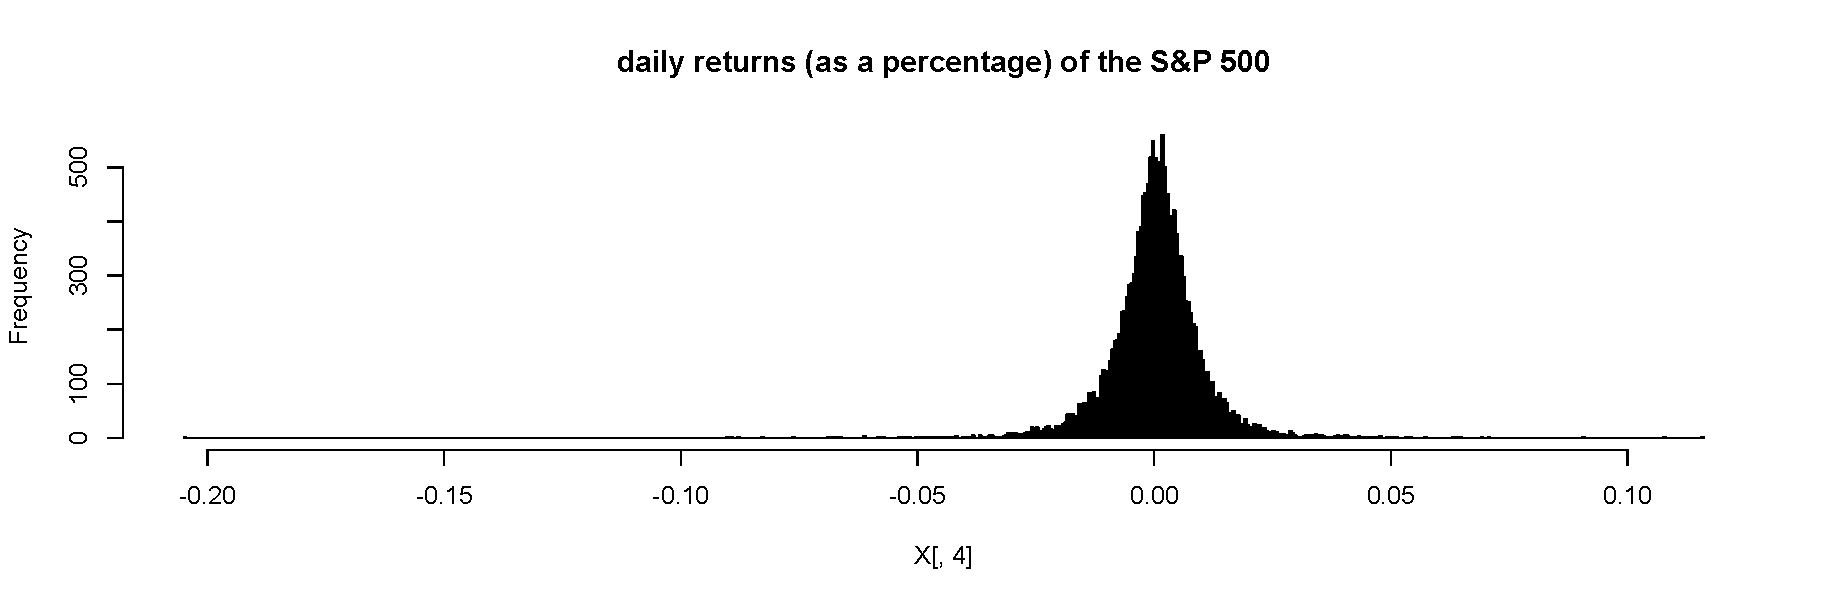
\includegraphics[width=7in]{daily_returns}
\end{figure}

\begin{verbatim}
X = read.csv('sp_tot_ret_price_1950.csv')
n = nrow(X)
n
hist(X[,4], br = 1000, 
  main = 'daily returns (as a percentage) of the S&P 500')
\end{verbatim}

\intermediatesubproblem{Regardless of normality, do you think the data is exchangeable?}\spc{4}

\intermediatesubproblem{Assume exchangeability and normality regardless of what you wrote in (a) and (b). The sample average is $\xbar=$0.0003415 and the sample standard deviation is $s=$0.0096. Under a relatively objective prior, give a 95\% credible region for the true mean daily return.}\spc{4}

\intermediatesubproblem{Give a 95\% credible region for \emph{tomorrow's} return.}\spc{15}

\intermediatesubproblem{Below is a sample of the same $n$ from the posterior predictive distribution in blue graphed atop the actual data in red (and a zoomed view of the tail). Is our model a good fit? Yes/no and explain.}\spc{2}

\begin{figure}[h]
\centering
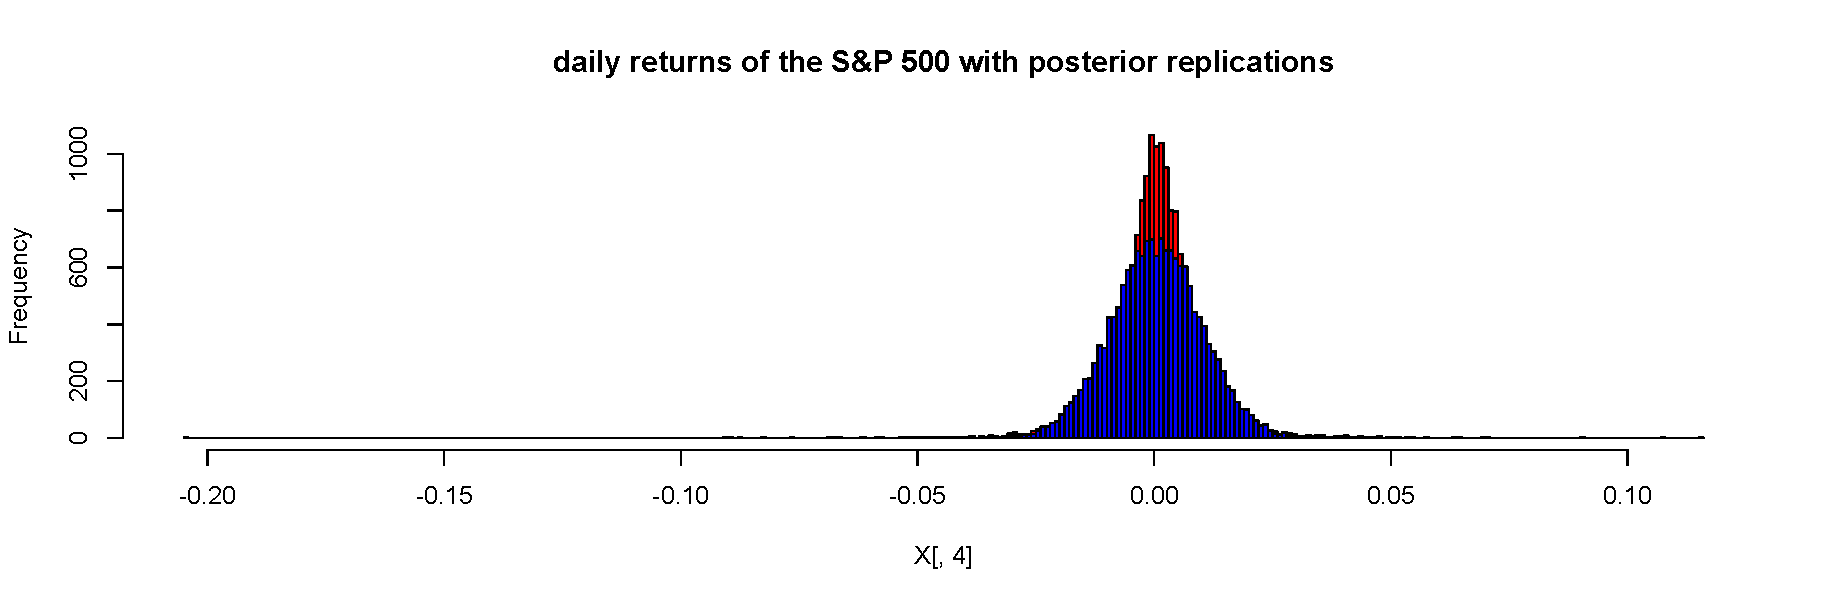
\includegraphics[width=7in]{daily_ret_post}
\end{figure}

\begin{verbatim}
hist(X[,4], br = 450, 
  main = 'daily returns of the S&P 500 with posterior replications', 
  col='red', xlim = c(-.1, -.02), ylim = c(0, 150))
hist(rnorm(16428, 0.0003415, 0.0096), br = 100, add = TRUE, 
  col = 'blue', xlim = c(-.1, -.02), ylim = c(0, 150))
\end{verbatim}

\begin{figure}[h]
\centering
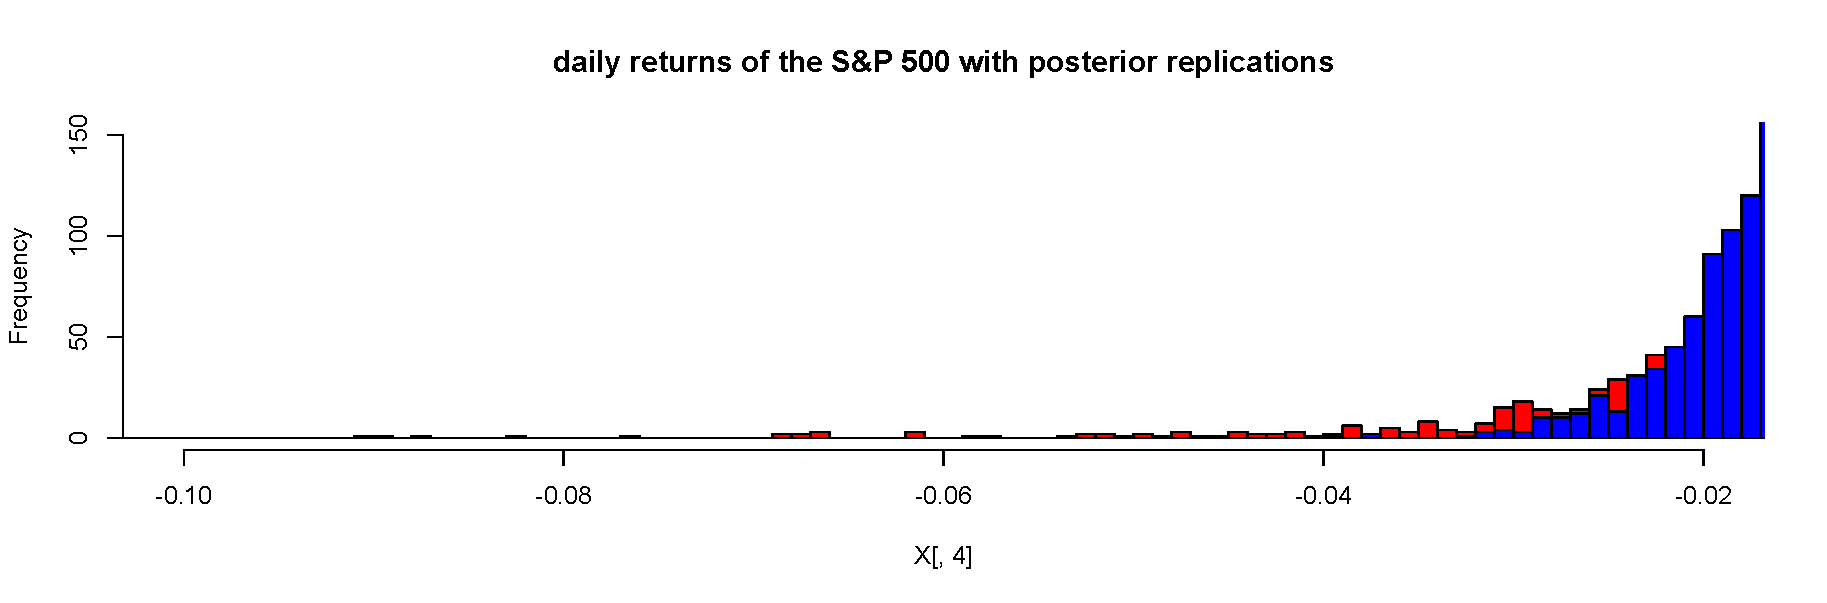
\includegraphics[width=7in]{zoom}
\end{figure}
\end{enumerate}
\end{document}




\problem{These are questions about McGrayne's book, chapters 11 and 12.}

\begin{enumerate}

\easysubproblem{Did Savage like Shlaifer? Yes / No and why?}\spc{3}

\easysubproblem{How did Neyman-Pearson approach statistical decision theory? What is the weakness to this approach? (p145)}\spc{3}

\easysubproblem{Who popularized \qu{probability trees} (and \qu{tree flipping}) similar to exercises we did in Math 241?}\spc{1}

\easysubproblem{Where are Bayesian methods taught more widely than any other discipline in academia?}\spc{2}

\easysubproblem{Despite the popularity of his Bayesian textbook on business decision theory, why didn't Schlaifer's Bayesianism catch on in the real world of business executives making decisions?}\spc{3}

\easysubproblem{Why did the pollsters fail (big time) to predict Harry Truman's victory in the 1948 presidential election?}\spc{2}

\easysubproblem{When does the diference between Bayesianism and Frequentism grow \qu{immense}?}\spc{3}

\easysubproblem{How did Mosteller demonstrate that Madison wrote the 12 Federalist papers of unknown authorship?}\spc{3}

\end{enumerate}


\problem{We will ask some basic problems on Empirical Bayesianism.}

\begin{enumerate}

\easysubproblem{Explain the methodology of Empirical Bayes the best as you can.}\spc{6}

\hardsubproblem{In what situations do you think Empirical Bayes methods work the best?}\spc{2}

\end{enumerate}



\problem{We will again be looking at the beta-prior, negative-binomial-likelihood Bayesian model. But first consider the more basic case where $\Xoneton \exchdist \geometric{\theta}$ and $\theta \sim \stdbetanot$.}


\begin{enumerate}


\easysubproblem{What is the likelihood model here? Write the PMF using the parameterization from class only.}\spc{2}

\intermediatesubproblem{Demonstrate that the posterior in this case is Beta and find the posterior parameters.}\spc{6}

\easysubproblem{Give expressions for $\thetahatmmse,~\thetahatmae$ and $\thetahatmap$ (use the approximation for the median of the beta distribution given in the notes for $\thetahatmae$). Are they all similar is $n$ is large?}\spc{3}

\hardsubproblem{Interpret the hyperparameters $\alpha$ and $\beta$ in the context of the posterior parameters.}\spc{5}



\easysubproblem{State the Jeffrey's prior for this model and explain why it is not proper.}\spc{2}

\easysubproblem{In what circumstances does Jeffrey's prior lead to a proper posterior?}\spc{2}

\easysubproblem{Given the posterior in (b), find the posterior in the case where you only observe one $x$.}\spc{2}

\hardsubproblem{You've seen the following data from the model: 5, 8, 6, 9, 11, 10, 7, 10, 11, 8, 9, 7, 7, 6. Design a prior using Empirical Bayes for $\theta$.}\spc{5}


\hardsubproblem{[MA] Use an objective prior. Imagine you now have seen 5 Bernoulli experiments go by with no success which you are patiently waiting for (since you can't use the cookie-cutter formulas until you see the success). Write an expression which if evaluated will provide the best guess of $\theta$ (best in a squared error loss sense) only given this \qu{partial} information. If you numerically compute it, you should get approximately 0.0238.}\spc{6}

%xs = seq(0, 100000)
%sum = 0
%alpha = 1
%beta = 1
%
%for (x in xs){
%	sum = sum + (alpha + 1)/(alpha+beta+1 + x) * beta(alpha + 1, x + beta) / beta(alpha, beta) 
%}
%sum


\intermediatesubproblem{Consider $\Xoneton \exchdist \negbin{r}{\theta}$ where $r$ is considered known and $\theta \sim \stdbetanot$ Demonstrate that the posterior in this case is Beta and find the posterior parameters.}\spc{6}

\easysubproblem{Give expressions for $\thetahatmmse,~\thetahatmae$ and $\thetahatmap$ (use the approximation for the median of the beta distribution given in the notes for $\thetahatmae$). Are they all similar is $n$ is large?}\spc{3}


\easysubproblem{[MA] Find the Jeffrey's prior for $\theta$ as a function of $r$. Look up the $I(\theta)$ on the Internet for the negative binomial given the parameterization we used in class. You do not need to do the derivation yourself.}\spc{2}

\hardsubproblem{[MA] Derive the posterior distribution PMF for one new negative binomial observation after seeing $n$ observations. This is a lot of computation.}\spc{18}

\hardsubproblem{[MA] Write an integral expression for the joint posterior distribution for $m$ new negative binomail observations. Extra credit if you can find the solution somewhere on the Internet.}\spc{6}

\intermediatesubproblem{Derive the PMF of the BetaGeometric($\alpha, \beta$) distribution. Hint: the formula for the BetaNegativeBinomial($r, \alpha, \beta$) PMF was given in class. All you need to do is solve for the special case when $r=1$. Leave in terms of the beta function.}\spc{5}

\intermediatesubproblem{Find the kernel of the BetaGeometric distribution.}\spc{6}


\intermediatesubproblem{Imagine $r=3$ and you've seen the following data from the model: 5, 8, 6, 9, 11, 10, 7, 10, 11, 8, 9, 7, 7, 6. Find an expression for the probability the next observation will be 10.}\spc{3}

\easysubproblem{Evaluate the probability in (q).}\spc{2}

\end{enumerate}


\problem{We will ask some basic problems on the Gamma-Poisson conjugate model.}

\begin{enumerate}

\easysubproblem{If $X \sim \poisson{\theta}$, what is the kernel of $\theta~|~X$?}\spc{2}

\easysubproblem{Write the PDF of $\theta$ which is the gamma distribution with the standard hyperparameters we used in class.}\spc{1}

\easysubproblem{What is the support and parameter space?}\spc{2}

\easysubproblem{What is the expectation and standard error and mode?}\spc{2}


\easysubproblem{Draw four different pictures of different hyperparameter combinations to demonstrate this model's flexibility}\spc{8}


\intermediatesubproblem{Prove that the Poisson likelihood for $n=1$ with a gamma prior yields a gamma posterior and find its parameters.}\spc{4}

\intermediatesubproblem{Prove that the Poisson likelihood for $n$ observations with a gamma prior yields a gamma posterior and find its parameters.}\spc{8}

\intermediatesubproblem{For the Poisson likelihood for $n$ observations with a gamma prior find $\thetahatmmse$, $\thetahatmae$ and $\thetahatmap$.}\spc{2}

\intermediatesubproblem{Demonstrate that $\thetahatmmse$ is a shrinkage estimator and find $\rho$.}\spc{4}

\easysubproblem{Demonstrate that $\prob{\theta} \propto 1$ is improper.}\spc{2}

\easysubproblem{Demonstrate that $\prob{\theta} \propto 1$ can be created by using an improper Gamma distribution (i.e. a Gamma distribution with parameters that are not technically in its parameter space and thereby does not admit a distribution function).}\spc{2}

\easysubproblem{What is the Jeffrey's prior for the Poisson likelihood model?}\spc{2}

\easysubproblem{What is the equivalent of the Haldane prior in the Binomial likelihood model for the Poisson likelihood model?}\spc{2}

\intermediatesubproblem{[MA] Prove that posterior predictive distribution for the next exchangeable Poisson realization given $n$ observed Poisson realizations is negative binomially distributed and show its parameters are $p = \beta / (\beta + 1)$ and $r = \alpha$ for $\alpha \in \naturals$.}\spc{10}

\hardsubproblem{If $\alpha \notin \naturals$, create an \qu{extended negative binomial} r.v. and find its PMF.}\spc{5}


\easysubproblem{Why is the extended negative binomial r.v. also known as the gamma-Poisson mixture distribution?}\spc{3}

\extracreditsubproblem{[MA] Find the joint posterior predictive distribution for $m$ future observations. I couldn't find the answer to this myself nor compute the integral.}\spc{5}

\intermediatesubproblem{If you observe $0,3,2,4,2,6,1,0,5$, give a 95\% CR for $\theta$. Pick an objective prior.}\spc{5}

\intermediatesubproblem{Using the data and the prior from (r), test if $\theta < 2$.}\spc{8}


\hardsubproblem{[MA] We talked about that the negative binomial is an \qu{overdispersed} Poisson. Show that the negative binomial converges to a Poisson. Try yourself before you Google the answer.}\spc{5}

\end{enumerate}


\problem{We will ask some basic problems on the Gamma-Exponential conjugate model.}

\begin{enumerate}

\easysubproblem{If $X \sim \exponential{\theta}$, what is the kernel of $\theta~|~X$?}\spc{2}

\intermediatesubproblem{Prove that the Exponential likelihood for $n=1$ with a gamma prior yields a gamma posterior and find its parameters.}\spc{8}

\intermediatesubproblem{Prove that the exponential likelihood for $n$ observations with a gamma prior yields a gamma posterior and find its parameters.}\spc{6}

\intermediatesubproblem{For the exponential likelihood for $n$ observations with a gamma prior find $\thetahatmmse$, $\thetahatmae$ and $\thetahatmap$.}\spc{2}

\intermediatesubproblem{Demonstrate that $\thetahatmmse$ is a shrinkage estimator and find $\rho$.}\spc{4}

\intermediatesubproblem{Use an uninformative prior like in the previous question. What is the posterior?}\spc{5}

\intermediatesubproblem{Write the integral to solve for the posterior predictive distribution for a single observation given $n$ observed data points.}\spc{5}

\hardsubproblem{[MA] Solve the integral.}\spc{6}

\extracreditsubproblem{[MA] Find the joint posterior predictive distribution for $m$ future observations.}\spc{0.1}

\hardsubproblem{[MA] What is the Jeffrey's prior for the exponential likelihood? Try yourself before you Google the answer.}\spc{5}

\end{enumerate}


\problem{We now begin the normal-normal conjugate model.}

\begin{enumerate}

\easysubproblem{If $X \sim \normnot{\theta}{\sigsq}$, what is the kernel of $\theta~|~X,~\sigsq$?}\spc{1}

\easysubproblem{If $X \sim \normnot{\theta}{\sigsq}$, what is the kernel of $\sigsq~|~X,~\theta$?}\spc{1}

\easysubproblem{If $X \sim \normnot{\theta}{\sigsq}$, what is the kernel of $\theta~,\sigsq~|~X$?}\spc{1}

\hardsubproblem{Show that posterior of $\theta~|~X,~\sigsq$ is normal if $\theta \sim \normnot{\mu_0}{\tausq}$. Try to do it yourself and only copy from the notes if you have to.}\spc{15}


\easysubproblem{What is the definition of the convolution of two r.v.'s $X_1$ and $X_2$?}\spc{1}

\hardsubproblem{Show that predictive distribution of $X^*~|~X,~\sigsq$ is normal if $\theta \sim \normnot{\mu_0}{\tausq}$ by solving the integral and not using the convolution.}\spc{12}

\hardsubproblem{Even though you solved this in (f), using the law of iterated expectation, find the expectation of the predictive distribution of $X^*~|~X,~\sigsq$.}\spc{8}

\hardsubproblem{Even though you solved this in (f), Using the law of total variance, find the variance of the predictive distribution of $X^*~|~X,~\sigsq$.}\spc{6}


\easysubproblem{In this problem we found the posterior, $\theta~|~X,~\sigsq$. What are all the other posteriors that could be of interest? Explain the inferential targets of each.}\spc{6}

\end{enumerate}


\end{document}
